\documentclass[a4paper,11pt]{article}
\pdfoutput=1 % if your are submitting a pdflatex (i.e. if you have
             % images in pdf, png or jpg format)

\usepackage{jinstpub} % for details on the use of the package, please
                     % see the JINST-author-manual
\usepackage[left]{lineno}
%\linenumbers %Turn on the line numbering for review
\title{Upgrades to the CMS Cathode Strip Chambers for the HL-LHC}


\abstract{The Large Hadron Collider (LHC) will be upgraded in several phases to significantly expand its physics program, and these upgrades present major challenges to the operations of the CMS Cathode Strip Chamber muon system. After the current long shutdown during 2018--2021 (LS2), the accelerator luminosity will have increased, exceeding the design value of $10^{34}$ cm$^{-2}$s$^{-1}$ and allowing the CMS experiment to collect approximately 100 fb$^{-1}$/year. A subsequent upgrade in 2023--2024 will increase the luminosity up to 5 x $10^{34}$ cm$^{-2}$s$^{-1}$. The CMS muon system must be able to sustain a physics program after the LS2 shutdown that maintains and enhances sensitivity to electroweak scale physics and for TeV scale searches similar to what was achieved up to now. For the Cathode Strip Chamber (CSC) muon  detectors, the electronics will be upgraded to handle the expected higher data rates.  The design of the upgraded CSC electronics is discussed in this report.  In addition, accelerated irradiation tests are being performed to study the behaviour of the CSC electronics under conditions that are nearly an order of magnitude beyond the original design values. Studies have also been performed of chamber gas mixtures to reduce greenhouse-gas impacts. The status of this irradiation campaign and results are presented.}



\keywords{Particle tracking detectors (Gaseous detectors), Wire chambers (MWPC), Muon spectrometers}


% \collaboration{\includegraphics[height=17mm]{example-image}\\[6pt]
%   XXX collaboration}
% or
\collaboration[a]{N. Manganelli on behalf of the CMS collaboration}
%\author[a]{N. Manganelli}
\affiliation{University of California, Riverside, USA}
\emailAdd{nicholas.james.manganelli@cern.ch}

\proceeding{IPRD2019: 15$^{th}$ Topical Seminar on Innovative Particle and Radiation Detectors\\
  October 14--17, 2019\\
  Siena, Italy}




\begin{document}
\maketitle
\flushbottom

\section{Introduction}
\label{sec:intro}
\paragraph{Cathode Strip Chambers}
The Compact Muon Solenoid (CMS) experiment \cite{detector}, located at Point 5 of the Large Hadron Collider (LHC), will contain 4 muon detector subsystems after Long Shutdown 2 (LS2) ends, each using different variants of gaseous detection technology.
In the forward region close to the beampipe, the Cathode Strip Chambers (CSCs) employ a multiwire proportional chamber (MWPC) design, providing both tracking and triggering information in the absolute pseudorapidity range 0.9--2.4.
The subsystem is comprised of 540 chambers partitioned into 2 endcaps with 4 disks per endcap and 2 to 3 rings per disk; each chamber is composed of 6 gas gaps with gold-plated tungsten wires sandwiched between two copper plates.
One copper plate is segmented into radial strips relative to the beampipe, and the wires are approximately perpendicular to the strips to facilitate measurements of the phi and radial coordinates of ionizing particles. The wires' angles from true perpendicular vary based on the magnetic field conditions where a particular chamber type is installed, which compensates for the differing charge drift angle. The working gas is 40\% argon, 50\% CO$_{2}$, and 10\% CF$_{4}$, where muons ionize the argon and the 2.9--3.6 kV potential induces e$^-$ and ion drift; e$^-$ avalanches form near the wires and corresponding image charges form on the cathodes (see figure \ref{fig:csc}). The subsystem contains a total of 266,112 cathode strips and 210,816 wire-groups that are read out by the front-end and back-end systems.
\begin{figure}[htbp]
\centering % \begin{center}/\end{center} takes some additional vertical space
%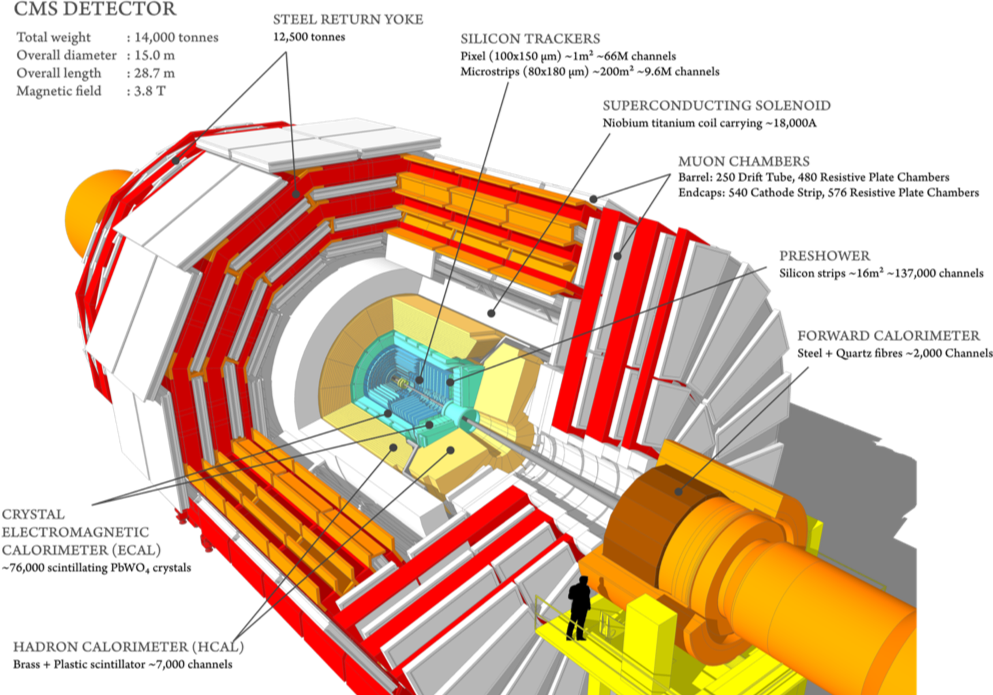
\includegraphics[width=.3\textwidth]{CMS.png}
%\qquad
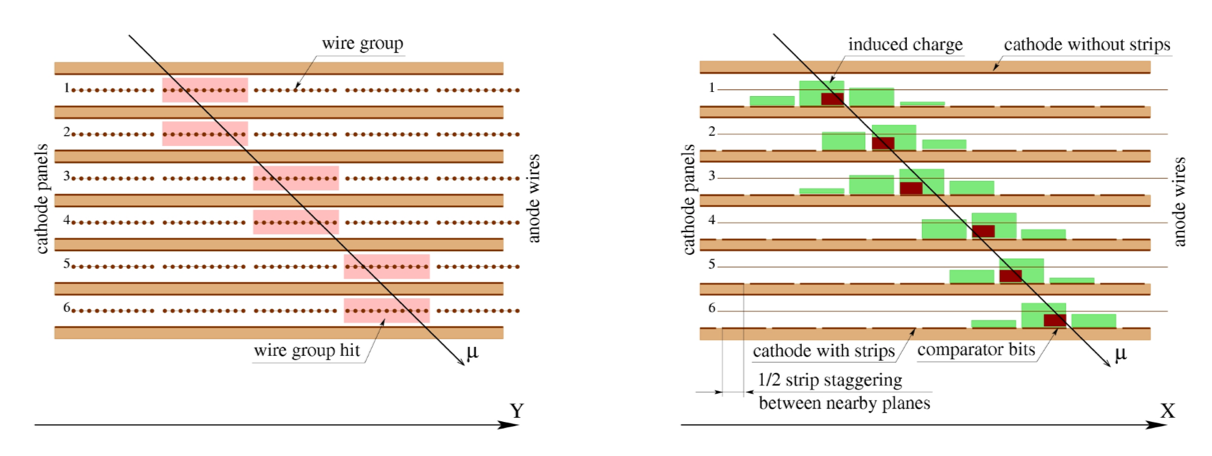
\includegraphics[width=1\textwidth]{CSC.png}
% "\includegraphics" from the "graphicx" permits to crop (trim+clip)
% and rotate (angle) and image (and much more)
\caption{\label{fig:csc} (left) Wire-group hits induced by muon ($\mu$), to be read out by the AFEBs and ALCT. (right) Cathode strip hits, to be read out by (x)(D)CFEBs.}
\end{figure}

\paragraph{Motivation for MWPC design}
The CSC design was chosen for the regions near the beampipe because of the following factors. First, it was necessary to use a technology that supports a high rate capability and very high efficiency, that has good performance over a range of background occupancies (up to 104 Hz/cm$^2$) and magnetic field conditions.
Additionally, the system needed good position resolution, acceptable time resolution, and the ability to provide tracking and triggering as part of a highly-redundant, high-longevity system.

\paragraph{On-chamber electronics}
The principal electronics installed on each chamber are the Anode Front End Boards (AFEBs), the Anode Local Charged Track (ALCT) mezzanine and baseboard, 
the Cathode Front End Boards (CFEBs), plus the Low Voltage Distribution Board (LVDB) and Motherboard (LVMB). The LVMB provides control and monitoring over power distribution, which is accomplished via the LVDB. The AFEBs are relatively simple readout devices connected to 16 wire groups each, 8 per layer; AFEBs connect to the ALCT baseboard, while the mezzanine houses the Fully Programmable Gate Array (FPGA) for determining the presence of ionization tracks in the wire-groups. The CFEBs are of greater complexity than AFEBs, with 96 strips from all 6 layers connected to each of the 4--7 boards; they contain amplifiers connected to strip readout, which feeds into flash ADCs for buffering of data and digital comparators to quickly identify potential ionization tracks in the strips. 

\begin{figure}[htbp]
\centering % \begin{center}/\end{center} takes some additional vertical space
\qquad
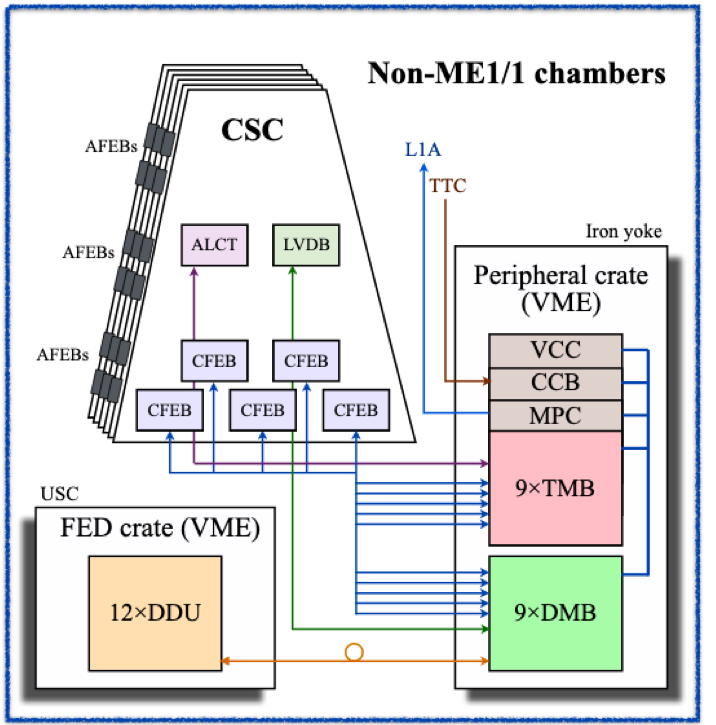
\includegraphics[width=.6\textwidth]{Electronics.png}
\caption{\label{fig:electronics} Layout of the on-chamber and off-chamber electronics. During LS2 the ALCTs, (D)CFEBs, and (O)TMBs are upgraded. During or before LS3, the (O)DMBs and FED system are upgraded. This figure is particular to non-ME1/1 chambers, with the principle differences being that ME1/1s have 7 Digital CFEBs and optical variants of the TMB and DMB \cite{tdr}.}
\end{figure}

\paragraph{Off-chamber electronics}
For each set of 9 chambers, there is one VME crate containing off-chamber electronics, located approximately a dozen meters from the furthest chambers and on the periphery of the CMS detector.
The Trigger Mother Board (TMB) receives triggering information from the ALCT and the DCFEBs, which it uses to create  potential local charged tracks (LCTs). If a coincidence in potential tracks is found between the anode wire-groups and cathode strips, the information is sent to higher level trigger systems for determining whether the CMS detector should do a complete event readout. In the case that such a signal is received back from the central triggering system (a so-called Level-1 Accept, or L1A), the
Data-Acquisition Mother Board (DMB) takes the more detailed data from CFEBs and ALCT (which have longer delays in the case of the former) and transmits them to the Front End Driver. For each chamber there exists a TMB/DMB pair. Per crate, there is also a 
VME Crate Controller (VCC) for control, monitoring, and firmware loading; a Clock and Control Board (CCB), which synchronizes the (sub-)system to LHC collisions; the Muon Port Card (MPC) is the path by which trigger info is sent to the more central systems (the next stage being the Endcap Muon Track-Finder). See figure \ref{fig:electronics}.

%\paragraph{Front End Driver electronics -- FED}
The Front-End Driver (FED), located in an underground service cavern (USC) near the CMS detector, contains Detector-Dependent Units (DDUs), which collect data from the DMBs and send them to an event builder computer farm. Each DDU collates input from 16 chambers from several disks using a staggered allocation, such that a muon passing through multiple in-line chambers has its information split amongst multiple DDUs.

\paragraph{Run II Performance}
The CSC subsystem maintained excellent stability and performance after nearly 200 fb$^{-1}$ integrated luminosity (instantaneous luminosity up to 2x10$^{34}$ Hz/cm$^2$). As seen in figure \ref{fig:runIIresolution}, the spatial resolution did not degrade between the 2017 and 2018 periods of Run II, and figure \ref{fig:runIIefficiency} shows the high efficiency of track reconstruction and trigger primitive creation for the 4 disks.
\begin{figure}[htbp]
\centering % \begin{center}/\end{center} takes some additional vertical space
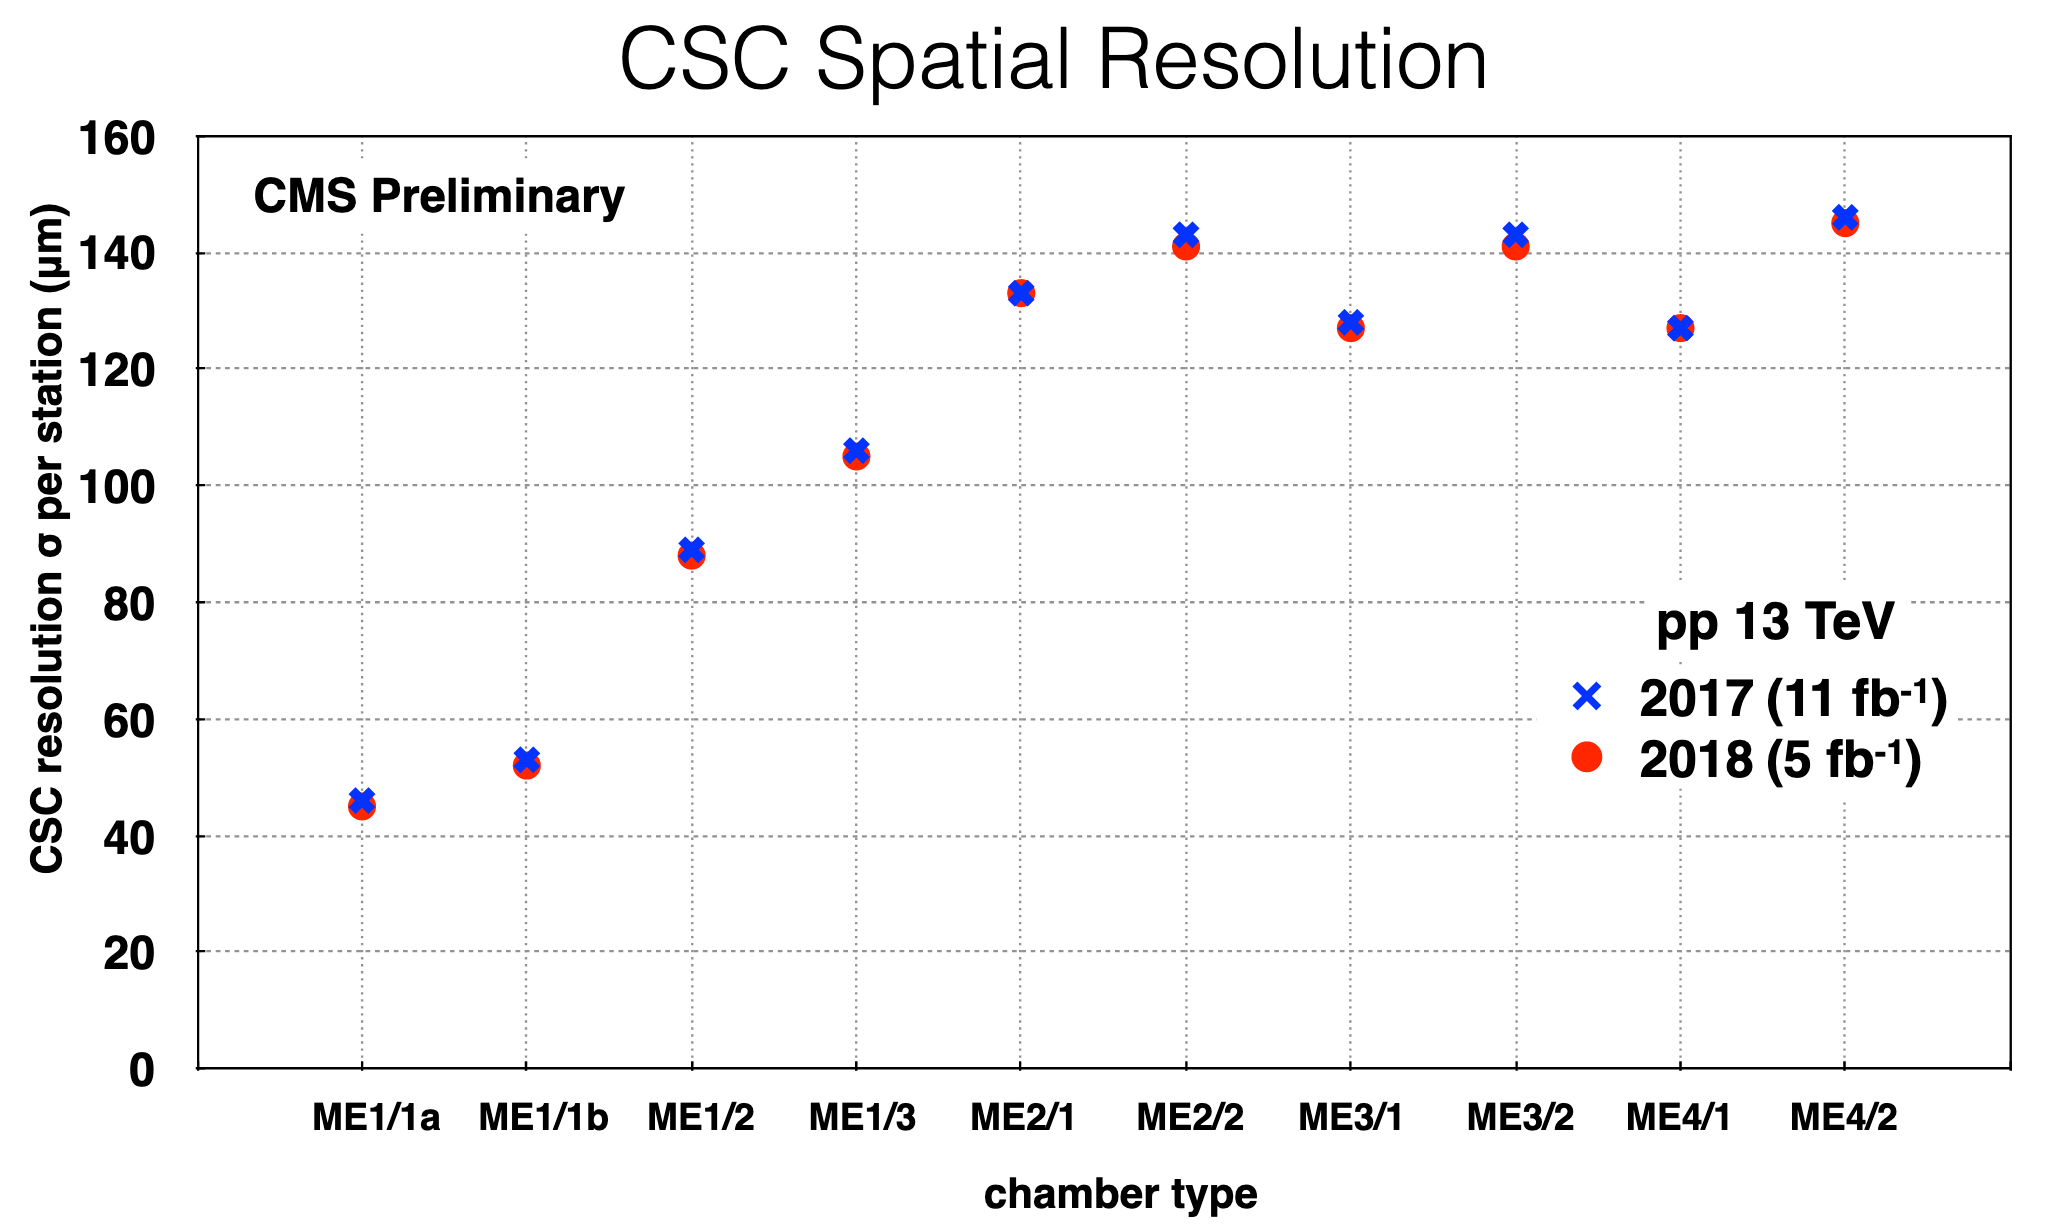
\includegraphics[width=.9\textwidth]{CSCSpatialResolution.png}
%\qquad
%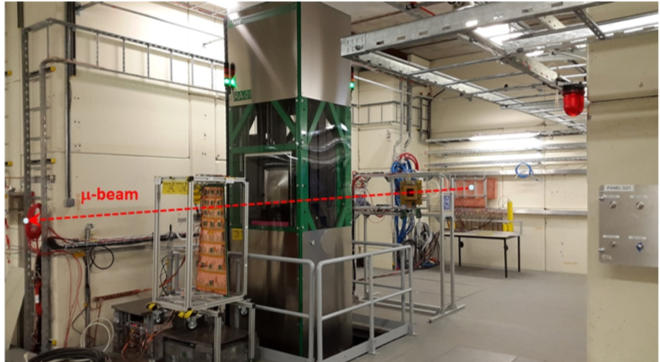
\includegraphics[width=.4\textwidth]{GIF.png}
\caption{\label{fig:runIIresolution} CSC Spatial resolution. The resolution shows no degradation between 2017 and 2018. Differences may be seen between different rings, and even between the two sections of ME1/1 chambers (these are denoted ME1/a and ME1/b) \cite{muonpublicresults}.}
\end{figure}

\begin{figure}[htbp]
\centering % \begin{center}/\end{center} takes some additional vertical space
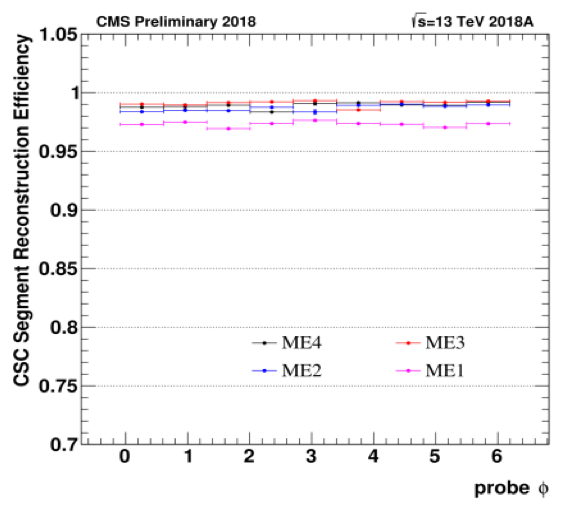
\includegraphics[width=.45\textwidth]{TrackEfficiency.png}
\qquad
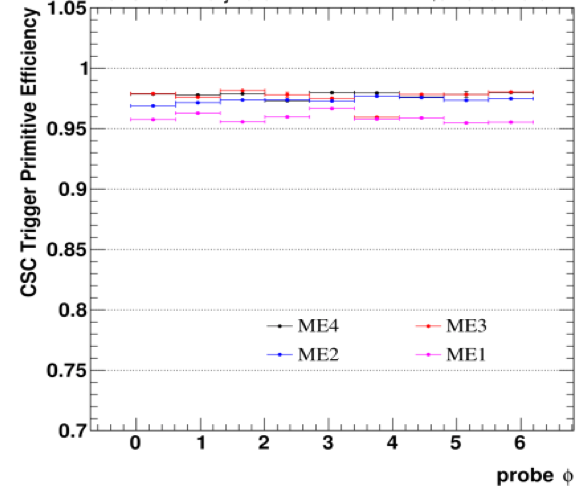
\includegraphics[width=.45\textwidth]{TriggerEfficiency.png}
\caption{\label{fig:runIIefficiency} (left) Track reconstruction efficiency of various CSC chamber types, ranging between 97\% and 99\% \cite{highlights}. (right) Trigger primitive efficiency, 96\% to 98\% \cite{highlights}.}
\end{figure}

\paragraph{Upgrade Motivation}
The principal goal of the High-Luminosity Large Hadron Collider project is to increase data collection by an order of magnitude (to 3000+ fb$^{-1}$), which necessitates a five-fold increase of the instantaneous luminosity (up to 7.5x10$^{34}$ Hz/cm$^2$) and thus more high-energy collisions and irradiation of sub-detectors.
%Higher average and peak number of proton-proton collisions per crossing-event (“pileup”)
The CMS collaboration will introduce the  Tracker subsystem to the Level 1 Trigger, which requires increasing latency to 12.5 $\mu$s, an increase by a factor of 3.5 over the Run II configuration. Besides the increased latency, the readout rate to the event builder server farm will also increase by a factor of 7.5 to 750 kHz. All of these factors mean that the CSC subsystem must maintain chamber performance in harsher conditions than the chambers were designed for and improve readout capability to match the longer latency and higher rates.

\section{Ensuring chamber longevity at the HL-LHC}
\label{sec:longevity}
\paragraph{Gamma Irradiation Facility (GIF++)}Given the particle rate and radiation increase for the HL-LHC, the CSC subsystem embarked on a campaign to test chamber performance and longevity to ensure good performance for the duration of the new physics program. CERN has commissioned the upgraded Gamma Irradiation Facility++ in order to test sub-detectors and their electronics in as realistic an environment as possible. This facility combines a muon beam up to 100--150 GeV/c with a $^{137}$Cs gamma source. GIF++ permits accelerated aging (up to 30x) and testing,
and can reasonably model a worst-case HL-LHC neutron-induced background where the CSCs are installed.
\paragraph{Projected HL-LHC performance and longevity}
Aging effects may manifest as changes in gas gain or the formation of dark currents. Si and C polymerization on wires can ruin uniformity and reduce the gas gain, which is the worst form of aging for a wire chamber. Additionally, continuous discharges may form (collectively dark currents), such as in the Malter Effect. See reference \cite{aging} for more details. Because of the focus on the anode, one way of characterizing wire chamber irradiation is via accumulated charge per unit length (of wire). After an exposure 3 times higher than expected for the HL-LHC program, no evidence for the development of strong dark currents was detected, and most importantly, there was only negligible change to the spatial resolution, as seen in figure \ref{fig:PerformanceHLLHC} \cite{highlights}. Within the limitations of accelerated aging tests, the results indicate the CSC subsystem can serve its function throughout the desired lifetime of the experiment.
\begin{figure}[htbp]
\centering % \begin{center}/\end{center} takes some additional vertical space
%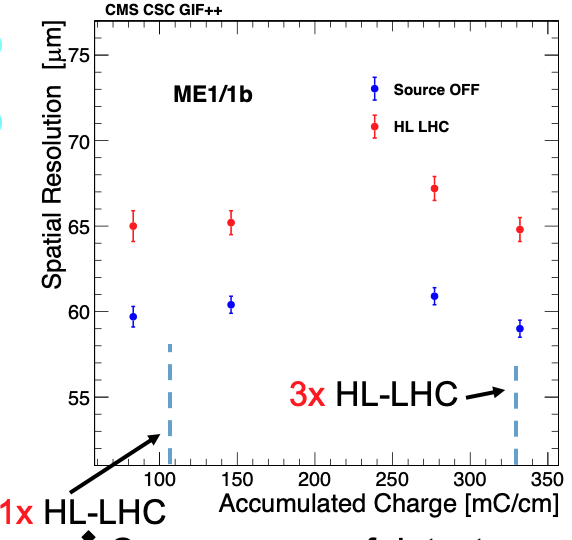
\includegraphics[width=.45\textwidth, trim=0 5 0 0, clip]{SpatialResolutionHLLHC.png}
\includegraphics[width=.45\textwidth]{GIF_Resol_vs_Q_11b_pnt_first_4p_tdrSt_HLLHC.png}
\qquad
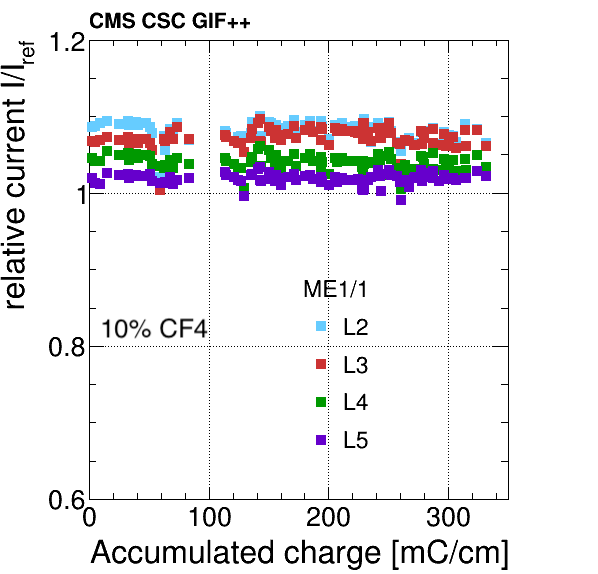
\includegraphics[width=.46\textwidth]{ME11_relI.png}
\caption{\label{fig:PerformanceHLLHC} (left) CSC spatial resolution up to 3x HL-LHC projected integrated luminosity. The lower points correspond to the Cs source being hidden, while the higher ones show the measurement of muon spatial resolution with the source actively simulating the neutron-induced background expected during HL-LHC operation \cite{hfo}. (right) Dark current, measured as a ratio to a reference current, with separate measurements in Layers 2--5 of a full-size chamber. No dark current formation is found up through 3x the HL-LHC lifetime \cite{highlights}.}
\end{figure}

\section{Reducing greenhouse gas consumption}
\label{sec:ghg}
\paragraph{Minimizing CF$_4$ content}
The nominal gas mixture performed well for chamber longevity in Run II. However, CF$_4$ has 6500x the global warming potential (GWP) of CO$_2$ (on a 100 year horizon), and acquisition of the gas is expected to become constrained. Studies undertaken with reduced CF$_4$ content show negligible aging and degradation through 3x HL-LHC accumulated charge as measured by gas gain losses and dark current formation. However, when the content is reduced to 2\%, there is visible surface darkening on the anodes, indicating surface pollution (see figure \ref{fig:PerformanceCF4Reduced}). As such, 5\% CF$_4$ is the lowest acceptable content, and a reduction to this level is not yet anticipated.
\begin{figure}[htbp]
\centering % \begin{center}/\end{center} takes some additional vertical space
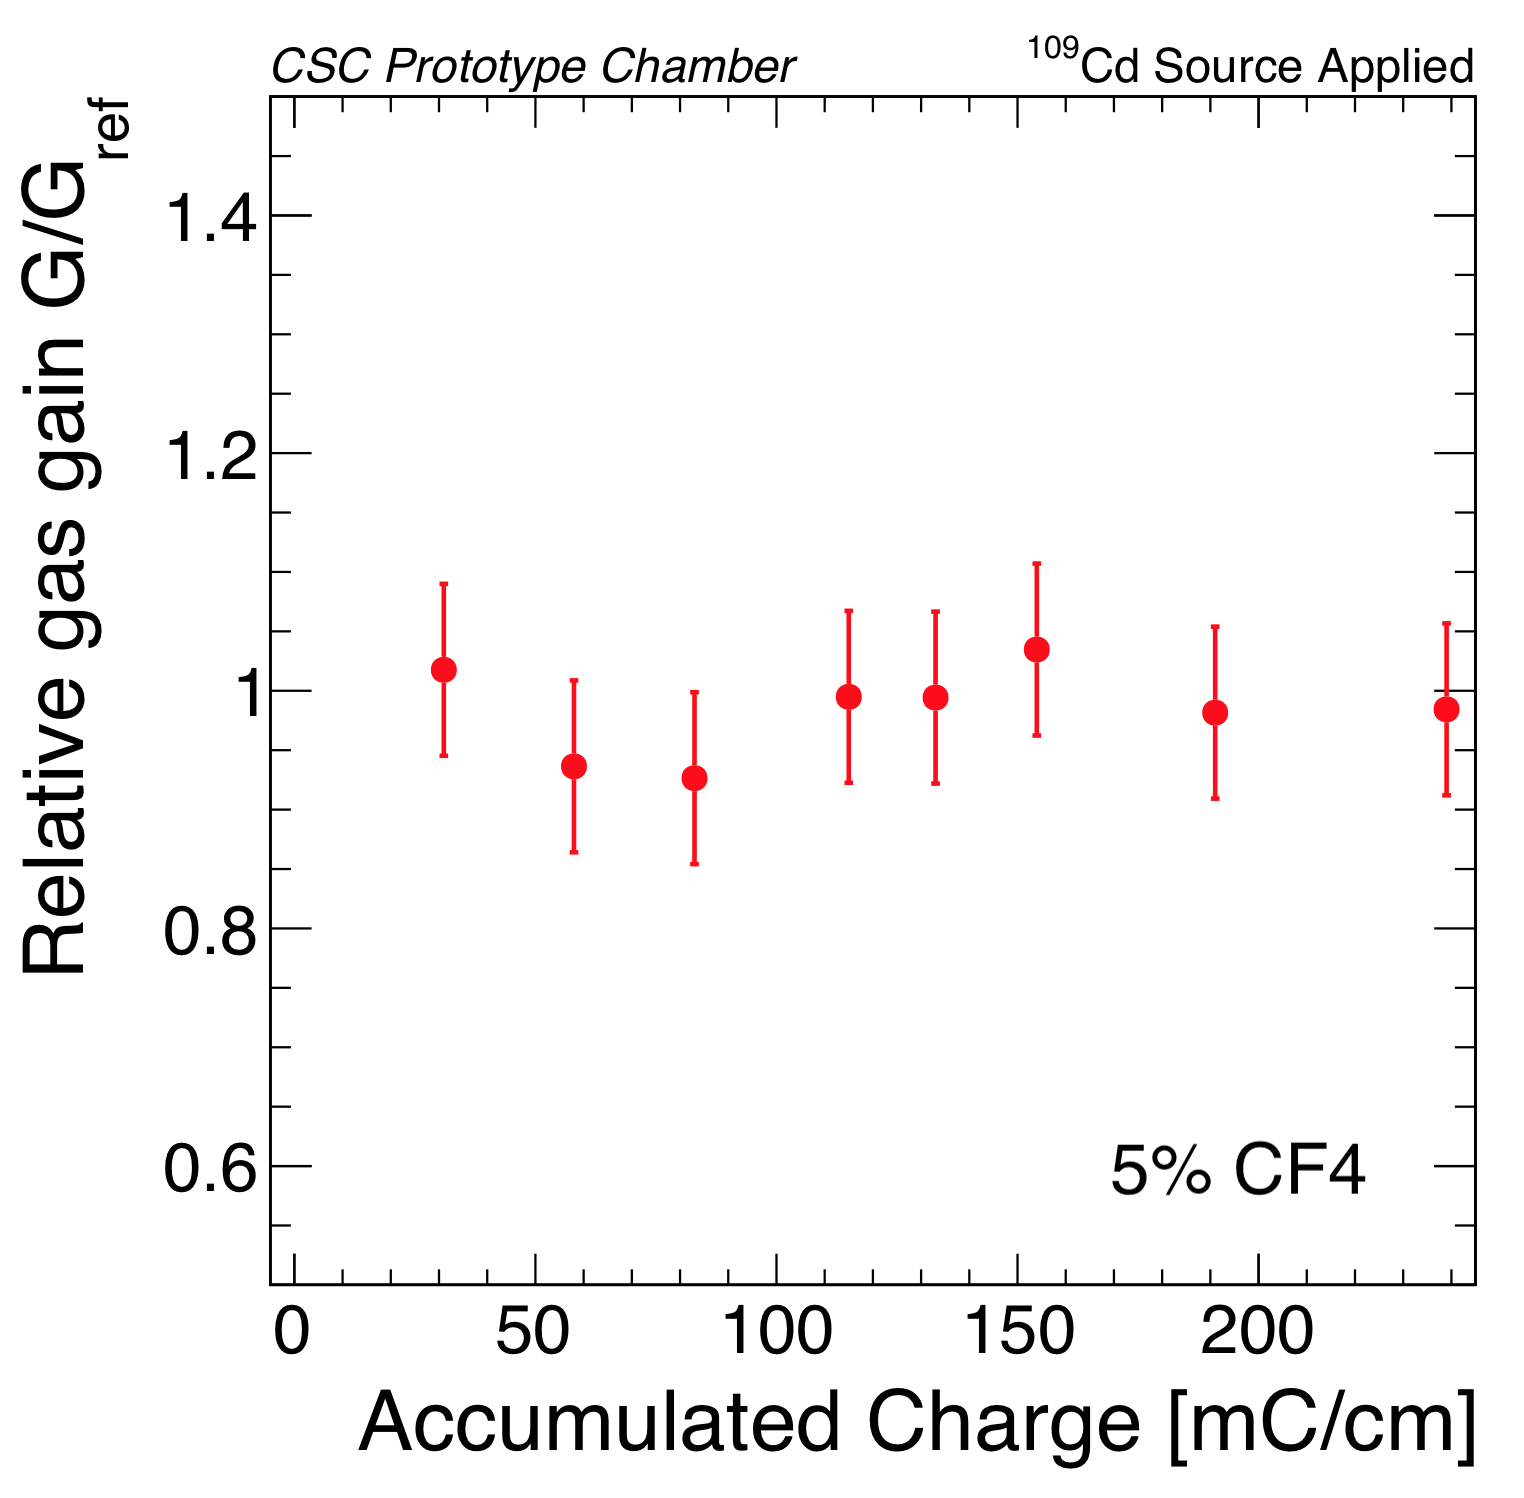
\includegraphics[width=.45\textwidth]{CSC-CF4-5Percent.png}
\qquad
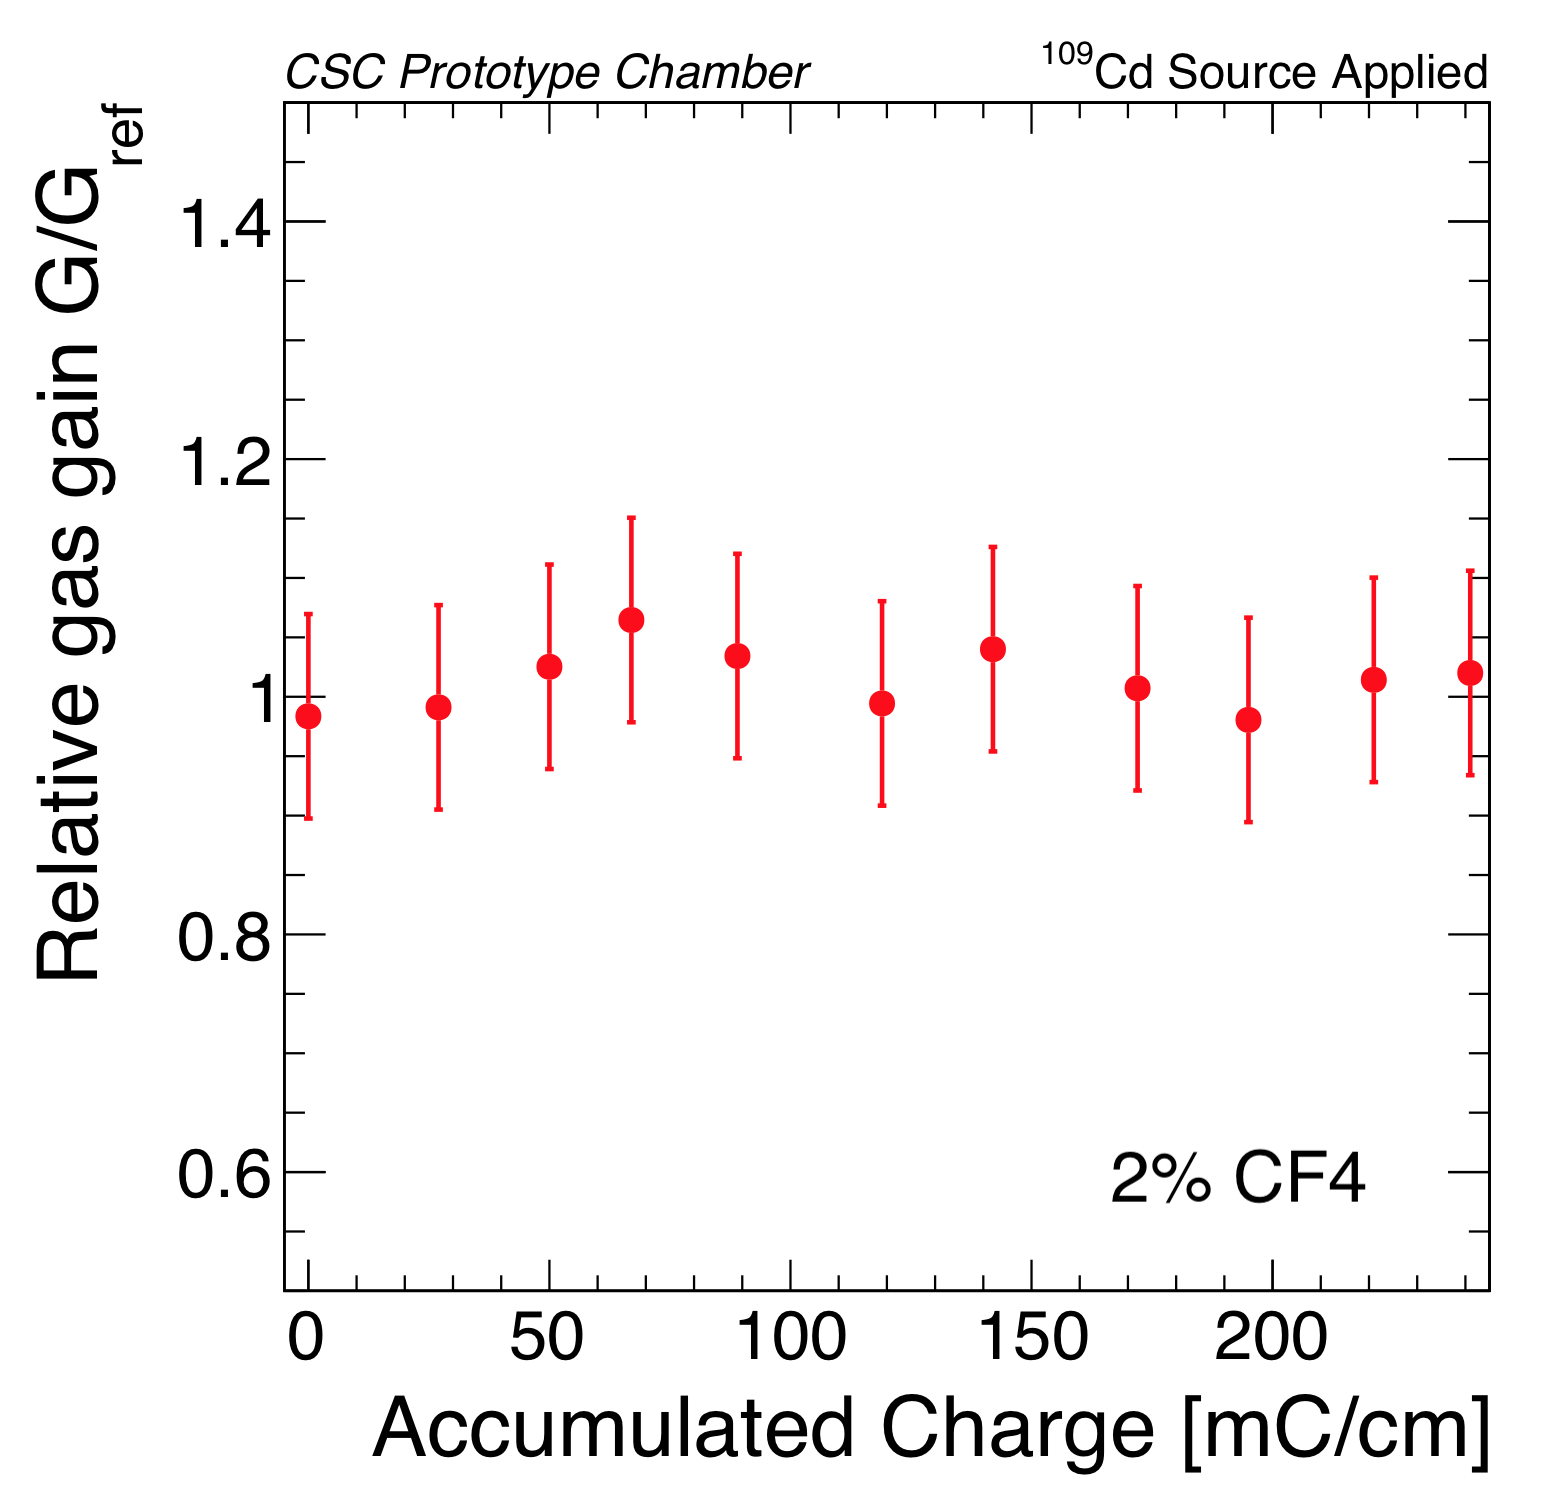
\includegraphics[width=.46\textwidth]{CSC-CF4-2Percent.png}
\qquad
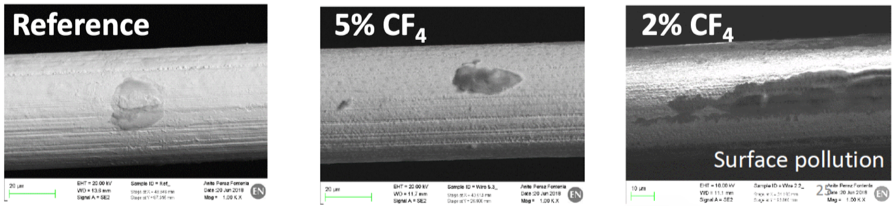
\includegraphics[width=.9\textwidth]{Pollution.png}
\caption{\label{fig:PerformanceCF4Reduced} (top) Gas gain with CF$_4$ reduced to 5\% and 2\%. No indication of aging is detected in this measurement \cite{reduction}. (bottom) Surface pollution with reduced CF$_4$, especially when dropped to 2\%, making such a reduction inadvisable \cite{reduction}.}
\end{figure}

\paragraph{Exploring CF$_4$ replacements}
Preliminary studies with one substitute for CF$_4$ that has a GWP less than 1, HFO-1234ze (HFO), show potential. 
The results visible in figure \ref{fig:PerformanceHFO} are the first in a CSC-type detector, HFO having been previously studied for Resistive Plate Chambers. 
An open gas loop in a 30 cm square prototype constructed with standard CSC materials was used.
Similar gas gain and drift velocities as 10\% CF4 are attainable with a 100 V high-voltage working point shift \cite{aging}. Measurements up through a safety factor of 10 were made, showing no significant degradation until more than 800 mC/cm (8x HL-LHC accumulated charge).
Further tests at GIF++ are scheduled with a full size chamber attached to a closed gas loop, where a slower acceleration factor will be used.
\begin{figure}[htbp]
\centering % \begin{center}/\end{center} takes some additional vertical space
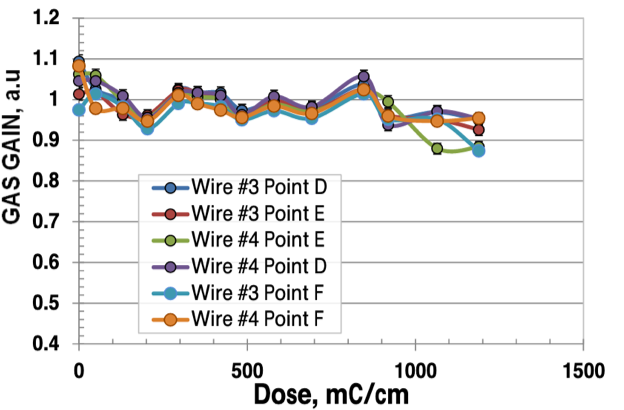
\includegraphics[width=.45\textwidth]{GainHFO.png}
\qquad
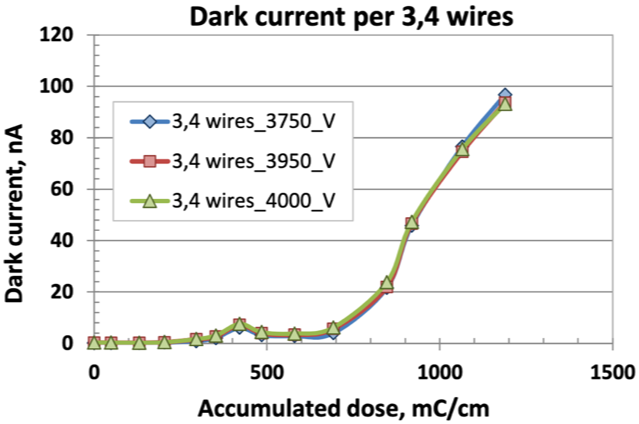
\includegraphics[width=.45\textwidth]{DarkCurrentHFO.png}
\caption{\label{fig:PerformanceHFO} (left) Gas gain with HFO replacing CF$_4$. Up through 800 mC/cm, there is negligible change to the gain, corresponding to almost 8 times the HL-LHC lifetime \cite{hfo} (right) Dark current, measured as a ratio to a reference current. No dark current formation is found until approximately 7 times HL-LHC lifetime. Wires 3, 4 refer to the ones closest to the local irradiation source in the prototype used for these tests \cite{hfo}.}
\end{figure}

\section{Electronics upgrades for the HL-LHC}
\label{sec:electronics}
\paragraph{Data losses at HL-LHC}
Due to the aforementioned increases to trigger and particle rates, drastic memory overflows and large readout inefficiencies/event losses are expected. In other words, the system needs to store more event data for a longer duration, then have access to more bandwidth to send them off-chamber. Figure \ref{fig:EventLoss} contains projections for the rings that will suffer the most, the ME2/1, ME3/1, and ME4/1 chambers. The ME1/1 chambers escape these losses as they received upgrades during Long Shutdown 1. The remaining CSCs closest to the beamline require upgraded on- and off-chamber electronics, and most must be installed in LS2 due to the schedule constraints of Long Shutdown 3 (just prior to the start of HL-LHC collisions).

\begin{figure}[htbp]
\centering % \begin{center}/\end{center} takes some additional vertical space
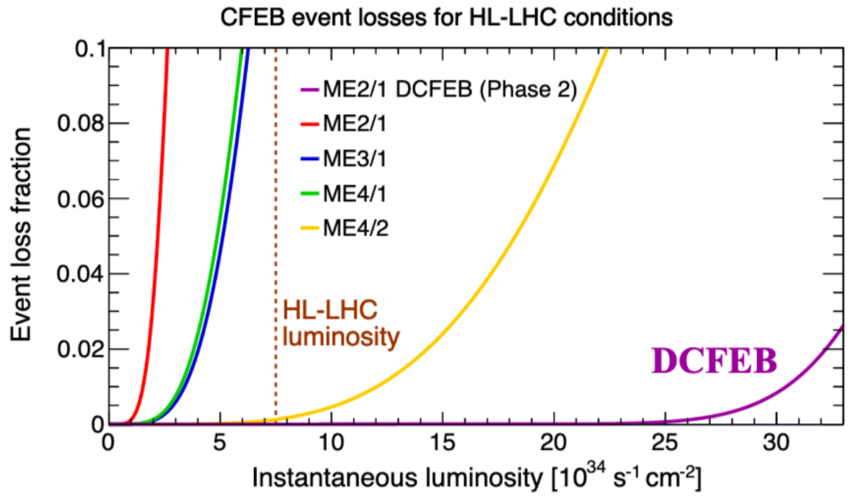
\includegraphics[width=.55\textwidth]{EventLoss.png}
\qquad
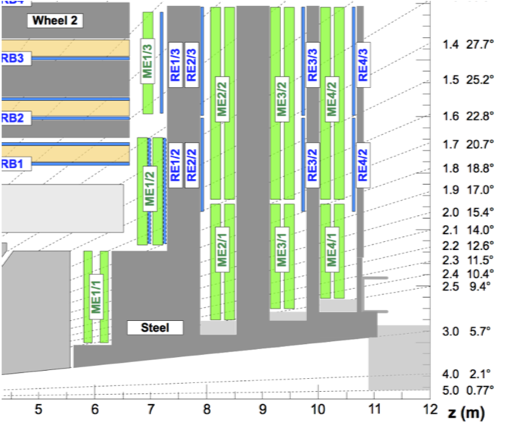
\includegraphics[width=.35\textwidth]{Diagram.png}
\caption{\label{fig:EventLoss} (left) The event losses for ME2/1, ME3/1, and ME4/1 chambers with CFEBs installed become drastic at the proposed HL-LHC luminosity. However, replacing CFEBs with upgraded Digital CFEBs as seen on the rightmost curve entirely mitigates the issue \cite{tdr}. (right) The interaction point is to the lower left, with the beamline along the z-axis. As can be seen, the ME1/1 is the least shielded from non-muons, while ME4/1 is the most shielded amongst the innermost rings \cite{performance}. }
\end{figure}

\paragraph{(x)DCFEB}
The Digital Cathode Front End Board (DCFEB) is an upgraded CFEB with a Virtex-6 FPGA, flash ADCs, digital pipeline (approximately 700 events deep), and 3.2 Gbps optical transmitters. These were designed and installed as an upgrade for ME1/1 chambers during Long Shutdown 1 (LS1); now they are being replaced and passed down to the ME2/1, ME3/1, and ME4/1 chambers. As a replacement for the DCFEBs being removed from ME1/1s, the xDCFEB (DCFEBv2) has been produced with CERN's radiation-hard Versatile Twin Transmitter (VTTx) and bidirectional Versatile Transceiver (VTRx) installed. A new capability to remotely program the FPGA via optical link and Gigabit Transceiver (GBTx) is included, providing a backup option in the event of EEPROM death due to the high radiation environment. Due to problems with the original optical transmitters on DCFEBs, they are retrofitted with VTTxs during the upgrade process, and 9 ME2/1 chambers received xDCFEBs instead of DCFEBs because there existed too few of the latter (accounting for spares) from the LS1 production.
\paragraph{ALCT}
Similar upgrades are necessary for the anode readout, in the form of new mezzanines.  Spartan-6 FPGAs are employed, with 9x--12x Block RAM of the original Virtex-E FPGAs. Optical transmitters provide 8x--12x the bandwidth of copper interconnects for the forward-most rings (ME1/1, 2/1, 3/1, 4/1). For chambers that read out 288--382 wire-groups, a smaller Spartan-6 is used; the ALCT-LX100 includes a VTRx when installed on ME1/1 chambers, supporting optical data readout to the new ODMB7 (4.48 Gbps) and EEPROM-less programming as in xDCFEBs. For the larger chambers, an ALCT-LX150T is installed, having FPGA resources for 576--672 wire-groups. A VTTx provides up to 6.4 Gbps data transmission to new ODMB5s, but until the ODMB5s are furnished after LS2, the old copper interconnects will suffice.

\paragraph{OTMB}
(x)DCFEBs output their trigger information through optical transmitters; thus they require an Optical TMB. The OTMBs designed and produced in 2013 for ME1/1 have been moved to peripheral crates for the ME3/1 and ME4/1 CSCs. The ME1/1 and ME2/1 crates will be outfitted with the new OTMB (2019) design in January 2020, which is almost identical to the 2013 version except for Samtec Firefly transceivers and the inclusion of inputs from the Gas Electron Multiplier (GEM) subsystem. These inputs allow synergy between the two subsystems once the GEMs are installed, as 
combining CSC and GEM trigger information increases efficiency and permits development of new triggering algorithms, such as for displaced muons. Additionally, in the forward-most regions the CSC chambers have been the only muon triggering system, and GEMs will provide redundancy for the HL-LHC program.

\paragraph{ODMB}
Chambers with (x)DCFEBs will receive new Optical DMBs by the time the HL-LHC starts operation. During Run III, prior to the installation of these boards, non-ME1/1 chambers with new on-board electronics will use the backwards-compatible copper interconnects to DMBs. The new ODMBs will come in two variants, ODMB5 for the ME2/1, ME3/1, and ME4/1 chambers that have 5 (x)DCFEBs, and an ODMB7 for the ME1/1 chambers (7 xDCFEBs each). A Kintex Ultrascale FPGA is the core of the new boards, with Firefly optical transceivers rated at 3.2 Gbps for the (x)DCFEBs and either a 4.8 Gbps bidirectional link for the ME1/1 ALCT or a dual 3.2 Gbps receiver for ALCT-LX150T mezzanines. To connect to the new FED, ODMB5s will use 2--3 10+ Gbps links, and ODMB7s will use 4 such links. As seen in figure \ref{fig:Bandwidth}, this results in a safety margin (between the expected and available bandwidths) of 3x to 6x for the 4 innermost rings of chambers, and chambers in the ME4/2 ring will have the smallest safety margin after the upgrade.
\begin{figure}[htbp]
\centering % \begin{center}/\end{center} takes some additional vertical space
%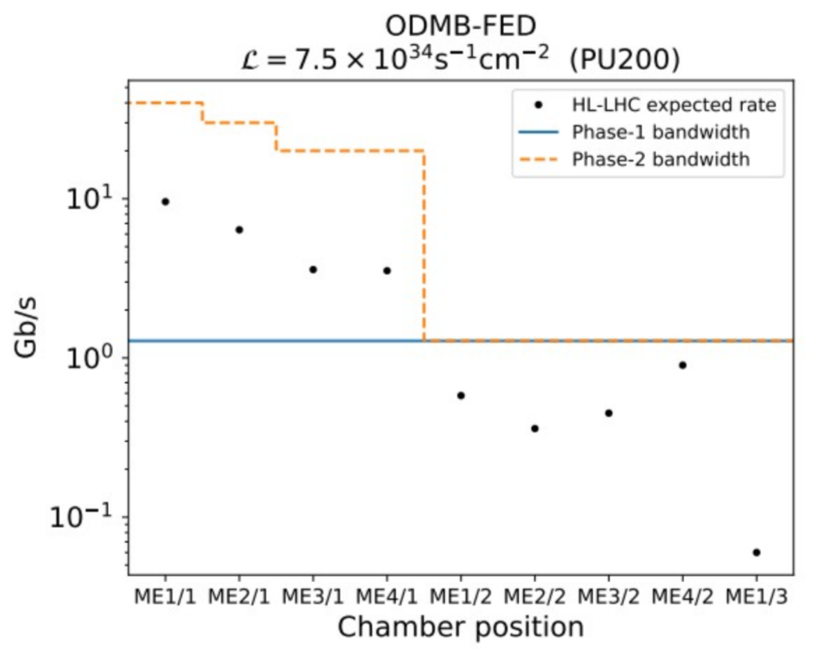
\includegraphics[width=.85\textwidth]{Bandwidth.png}
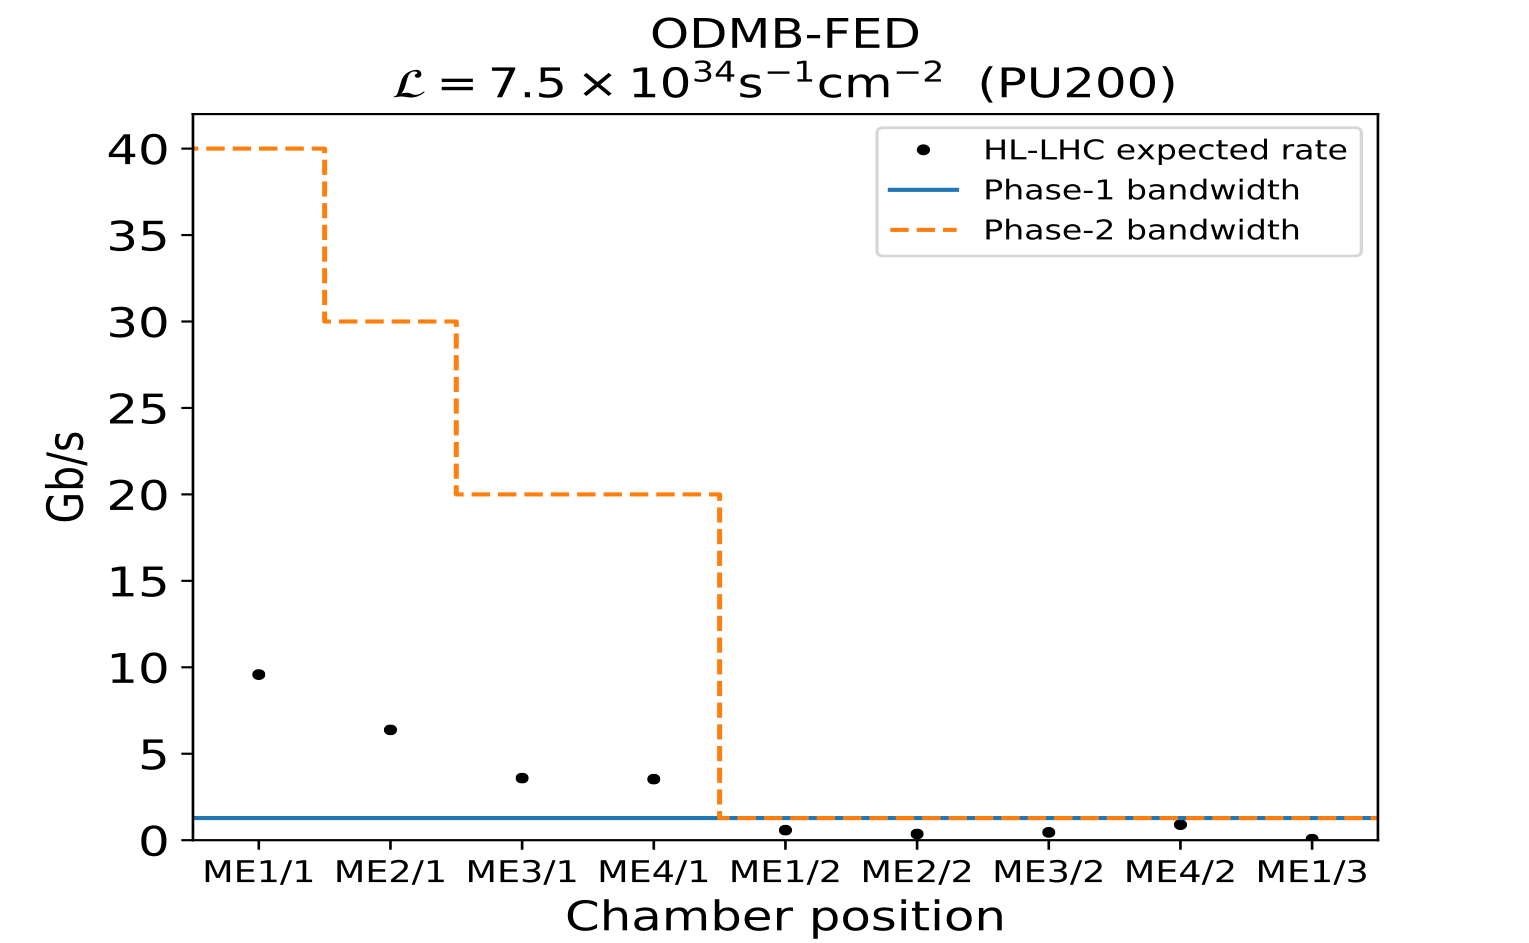
\includegraphics[width=.85\textwidth]{ODMB-FED-Lin.png}
\caption{\label{fig:Bandwidth} The Phase-2 bandwidth will exceed the projected HL-LHC needs by a small margin, with the increased bandwidth of ODMB7s and ODMB5s apparent versus the Phase-1 bandwidth. Four Links are available for ME1/1 ODMB7s, while ODMB5s are configured to use 2 or 3 links to the FED based on the ring for which they are installed. The figure is produced with an expected PileUp of 200 pp collisions per bunch crossing (PU200) [from personal correspondence with Jaebak Kim, Oct. 2, 2019].}
\end{figure}

\paragraph{FED}
During Long Shutdown 3 (LS3), starting in 2025, the FED will receive an upgrade coinciding with the new ODMBs. An industry standard, the Advanced Telecommunications Computing Architecture (ATCA) is common to many CMS upgrade projects. In particular, the CSCs will share the same processing module with parts of the new GEM muon sub-detector, which is being installed in stages during LS2 (GE1/1), LS3 (ME0), and in-between LS2 and LS3 (GE2/1). The shared module will consist of an APX Consortium card (APT) (figure \ref{fig:FED}) with 100 bidirectional links rated at 25 Gbps and a Virtex Ultrascale FPGA (VU9P currently). The total CSC Data Acquisition rate will be 1344 Gbps, an aggregate of chambers using DMBs with 1.6Gbps links, chambers with ODMB5s using 2--3 12.25 Gbps links, and 72 ME1/1 chambers using 4 12.25 Gbps links per ODMB7. At a minimum, 9 APT boards will make up the new FED system, replacing 36 DDUs. (Information from personal correspondence with Evaldas Juska, Oct. 8, 2019)
\begin{figure}[htbp]
\centering % \begin{center}/\end{center} takes some additional vertical space
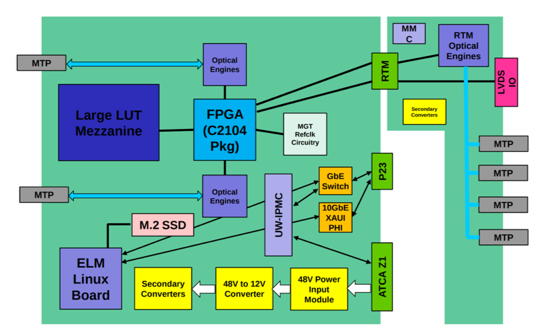
\includegraphics[width=.35\textwidth]{APTX.png}
\qquad
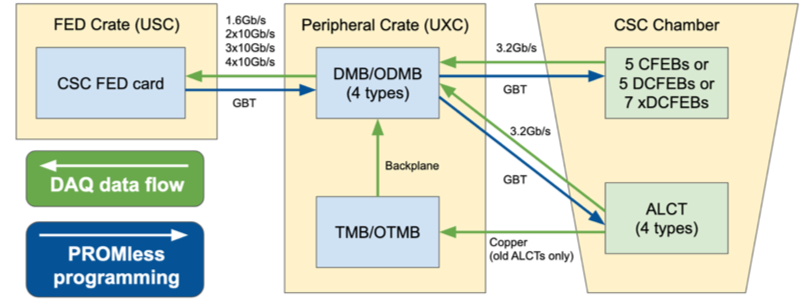
\includegraphics[width=.45\textwidth]{FED.png}
\caption{\label{fig:FED} (left) APX Consortium Card design \cite{fed}. (right) Layout of the system after electronics upgrades \cite{fed}.}
\end{figure}

%\paragraph{FIXME:Unused}
%All new electronics tested for both Total Irradiated Dose and Single Event Upset limits
\section{Conclusion}
\label{sec:conclusion}
\paragraph{}
Cathode Strip Chambers are a classic technology that provided all of the necessary ingredients for a successful muon tracking and triggering system in the CMS forward region.
The CSC subsystem has thus far demonstrated great performance and longevity with the original gas mixture and electronics.
To evaluate more eco-friendly options, studies are underway with reduced CF$_4$ and substitutes like HFO-1234ze.
Higher latency and event rates at the HL-LHC necessitate upgrades of on- and off-chamber electronics, the core tenets being more bandwidth (optical instead of copper links) and deeper buffers. These upgrades are underway currently, having successfully reached the halfway point of the LS2 schedule and scope.

\acknowledgments

Thanks to the many members of the CMS CSC community who contributed information, figures, and feedback, and without whom this document would not have been possible. 

\begin{thebibliography}{99}
\bibitem{detector} CMS Collaboration, \emph{The CMS Experiment at the CERN LHC}, \emph{JINST} {\bf 3} S08004 (2008)

\bibitem{tdr} CMS Collaboration,
\emph{The Phase-2 Upgrade of the CMS Muon Detectors: Technical Design Report},
CERN-LHCC-2017-012, \emph{CMS-TDR-016}

\bibitem{muonpublicresults}CMS Collaboration. \emph{Performance of the CMS Muon Detectors in Early 2018 Collision Runs}, 26 Sept. 2018, twiki.cern.ch/twiki/bin/view/CMSPublic/MuonDPGPublic180622

\bibitem{highlights}
Lenaro, A., \emph{CSC Highlights from 2018}, CMS General Muon Meeting, (Dec. 4, 2018)

\bibitem{aging}
Kadyk, J. A., \emph{Wire Chamber Aging}, \emph{Nucl. Instrum. Methods Phys. Res.} {\bf A300} (1991) pp 436--479

\bibitem{hfo}
Gavrilov, G., \emph{CSC Aging Studies and Future Plan/Milestones}, \emph{CMS Muon Upgrade Workshop} (Oct. 7--9, 2019)

\bibitem{reduction}
Wisecarver, A., \emph{Gas Mixture Longevity Studies for the CMS Cathode Strip Chambers in Preparation for HL-LHC}, 2019 APS Meeting of the Division of Particles \& Fields (2019)

\bibitem{performance}
CMS Collaboration, \emph{Performance of the {CMS} Muon Detector and Muon Reconstruction with Proton-proton Collisions at $\sqrt{}$s=13 {TeV}},
\emph{JINST} {\bf 13} (2018)
arXiv:1804.04528v2

\bibitem{fed}
Juska, E., \emph{Muon Backend Electronics Overview}, CMS Muon Annual Review, (Sept. 24, 2018)


% Please avoid comments such as "For a review'', "For some examples",
% "and references therein" or move them in the text. In general,
% please leave only references in the bibliography and move all
% accessory text in footnotes.

% Also, please have only one work for each \bibitem.


\end{thebibliography}
\end{document}
